\section{Question 2}
Halo orbits are a type of periodic orbit that occur in the three-body problem, where two massive celestial bodies exert gravitational forces on a third, much smaller body. These orbits are characterized by their peculiar shape, which resembles a three-dimensional figure-eight or a halo, hence the name.

The motion of a spacecraft in a halo orbit can be described by the Hill's equations, given by:

\begin{equation}
\ddot{\mathbf{r}} - 2\boldsymbol{\Omega}\times\dot{\mathbf{r}} - \boldsymbol{\Omega}\times(\boldsymbol{\Omega}\times\mathbf{r}) = \frac{{G(m_1 + m_2)}}{{r^3}}\mathbf{r}
\end{equation}

where $\mathbf{r}$ represents the position vector of the spacecraft, $\boldsymbol{\Omega}$ is the angular velocity vector of the reference frame, $m_1$ and $m_2$ are the masses of the primary bodies, and $G$ is the gravitational constant.

Halo orbits exist in the circular restricted three-body problem, where one of the primary bodies is considered massless. The Lagrange points $L_1$, $L_2$, and $L_3$ serve as stable equilibrium points for halo orbits. A halo orbit around $L_1$ or $L_2$ can be defined by specifying its amplitude $A$, in terms of the distance between the primary bodies $r_0$, and the period $T$.

The equation for the shape of a halo orbit can be written as:

\begin{equation}
x = A\cos(\theta + \phi_0), \quad y = A\sin(\theta + \phi_0), \quad z = 0
\end{equation}

where $x$, $y$, and $z$ represent the coordinates of the spacecraft in the rotating frame, $\theta$ is the true anomaly, and $\phi_0$ is the initial phase angle.

Halo orbits have been of great interest in space exploration, as they provide stable trajectories for spacecraft to observe and study various celestial bodies.


\subsection{Howell Method for Halo Orbits}

Halo orbits are periodic orbits that occur in the three-body problem, characterized by their peculiar shape resembling a three-dimensional figure-eight or a halo. The Howell formula and the iterative $\phi$-matrix method are two commonly used techniques to calculate halo orbits.

The Howell formula is an analytical expression that provides an approximation for the amplitude of a halo orbit. It is given by:

\begin{equation}
A = \left(\frac{{m_2}}{{3\Omega^2}}\right)^{1/3}\left(\frac{{r_0^2}}{{4}}\right)^{1/3}
\end{equation}

where $m_2$ is the mass of the secondary body, $\Omega$ is the angular velocity of the reference frame, and $r_0$ is the distance between the primary bodies.

However, the Howell formula only provides an estimate of the amplitude, and it does not give the full trajectory of the halo orbit. To obtain a more accurate representation, the iterative $\phi$-matrix method is often employed.

The iterative $\phi$-matrix method involves solving a set of coupled linear equations iteratively to obtain the $\phi$-matrix, which describes the linearized motion around the nominal halo orbit. The $\phi$-matrix is updated in each iteration until convergence is achieved.

The equation for updating the $\phi$-matrix is given by:

\begin{equation}
\phi_{k+1} = \frac{{\partial R(\tau)}}{{\partial y}} \bigg|_{y=y_k} \phi_k
\end{equation}

where $\phi_k$ represents the $\phi$-matrix at the $k$-th iteration, $R(\tau)$ is the state transition matrix, and $y_k$ is the state vector at the $k$-th iteration.

By iterating the above equation until convergence, the $\phi$-matrix is obtained, which can then be used to calculate the full trajectory of the halo orbit.

The Howell formula and the iterative $\phi$-matrix method are powerful tools for calculating halo orbits, providing approximations and accurate representations, respectively. These methods have been widely used in space mission design and celestial mechanics research.
 \subsection{Part a}
 Used Attached code for specific initial conditions and got the following results:
 \begin{table}
        \centering
        \begin{tabular}{|c|c|c|c|c|c|}
            \hline
            $X$ & $Y$ & $Z$ & $V_x$ & $V_y$ & $V_z$ \\
            \hline
            0.82411 & 0 & 0.05625356 & 0 & 0.166629 & 0 \\
            \hline
        \end{tabular}
        \caption{Halo orbit parameters}
 \end{table}

 \subsection{Part b}
 Used above attached code and got the following results:
 \begin{figure}[H]
    \centering
    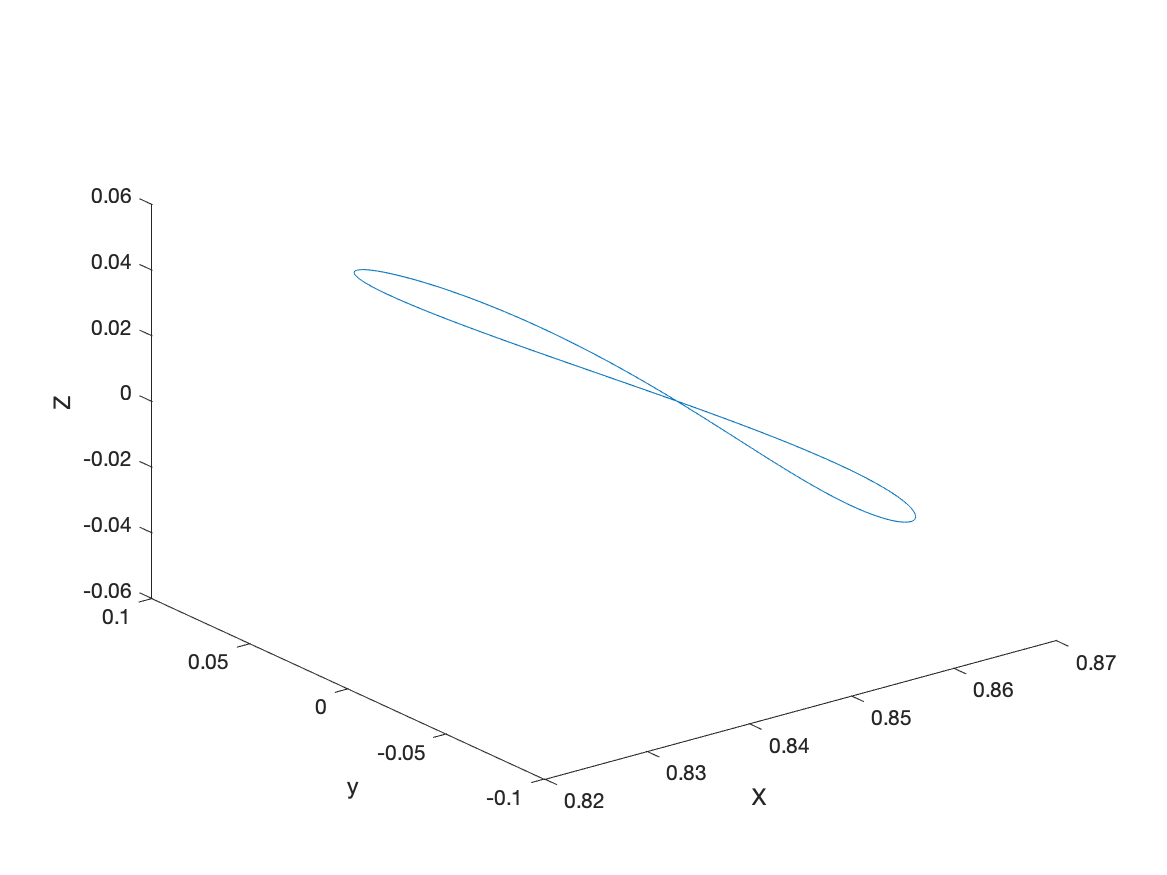
\includegraphics[width=\textwidth]{../Figure/Q2/fig1}
    \caption{Halo orbit in 3D}
\end{figure}

\begin{figure}[H]
    \centering
    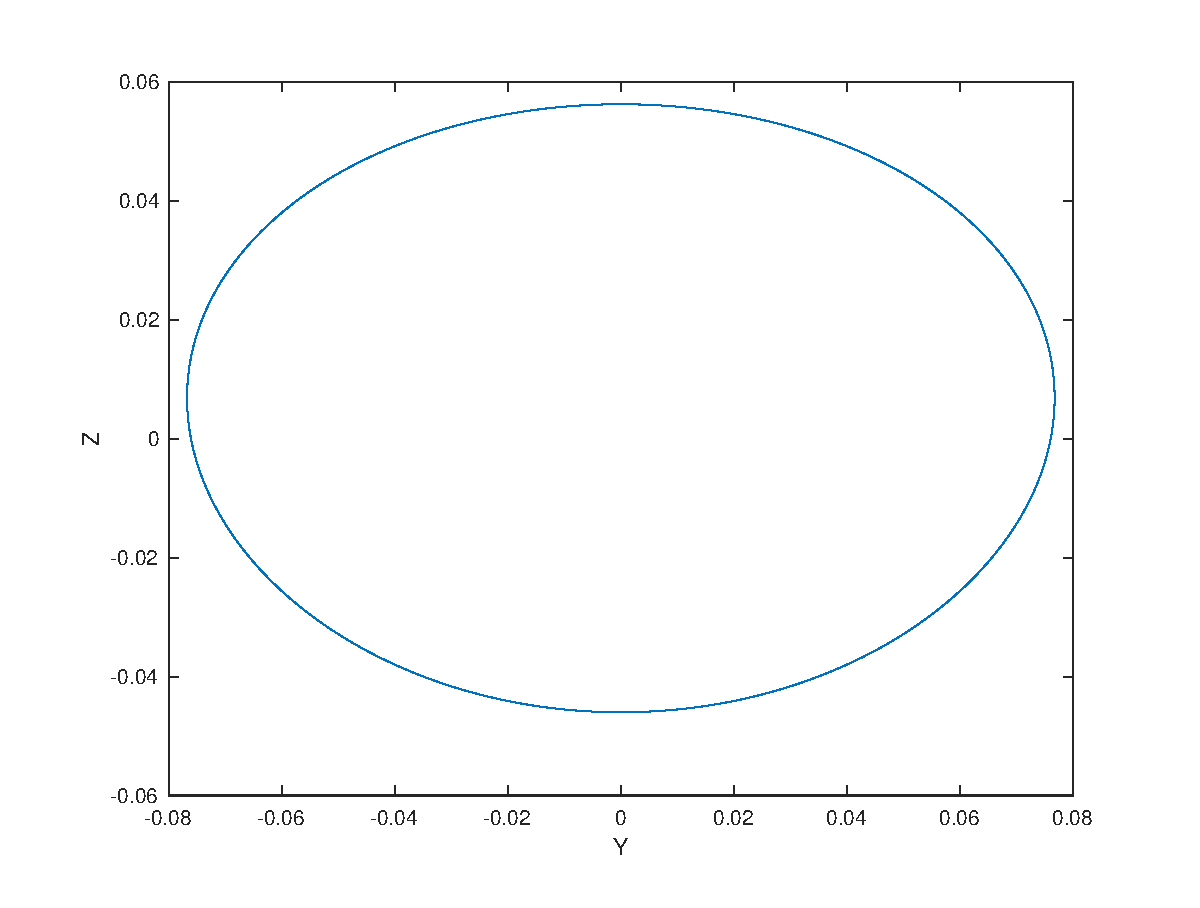
\includegraphics[width=\textwidth]{../Figure/Q2/fig2}
    \caption{Halo orbit in YZ plane}
\end{figure}

\begin{figure}[H]
    \centering
    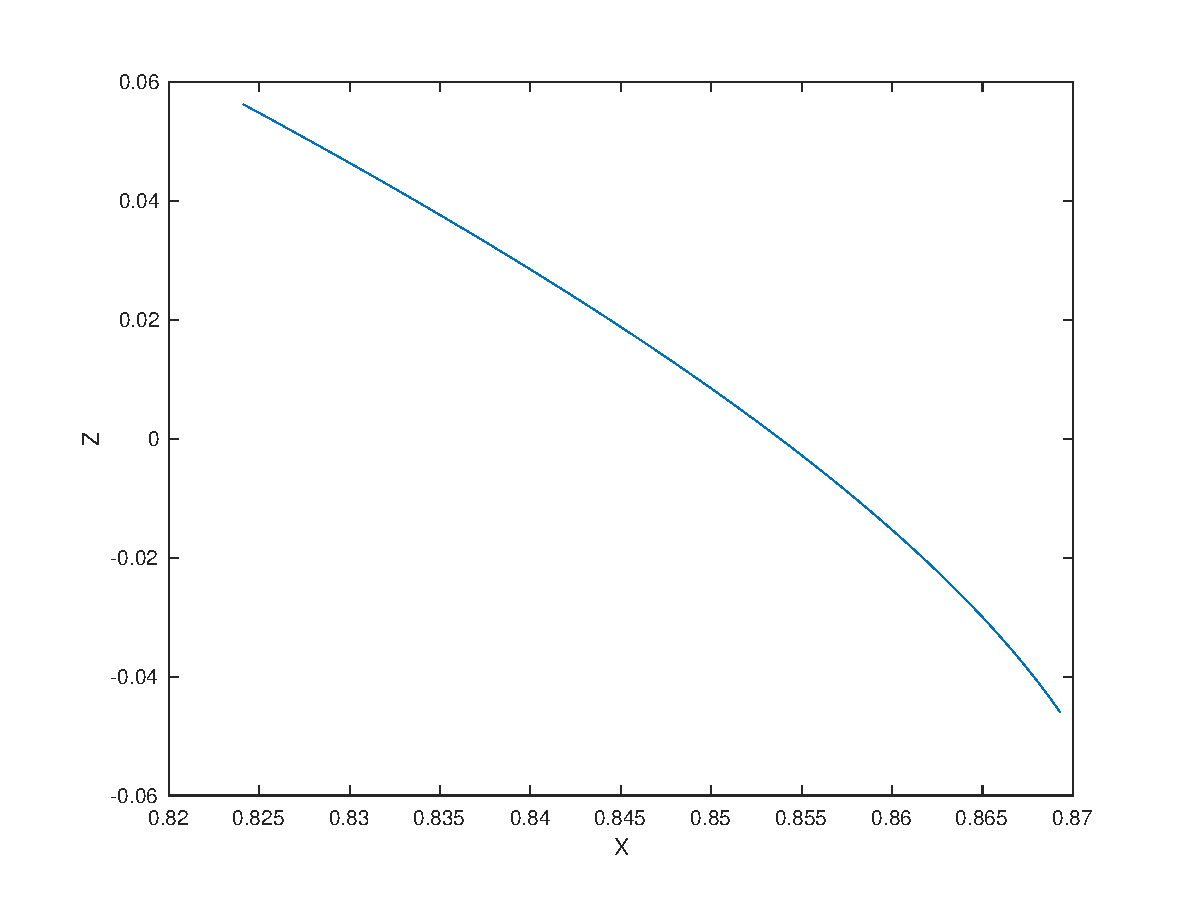
\includegraphics[width=\textwidth]{../Figure/Q2/fig3}
    \caption{Halo orbit in XZ plane}
\end{figure}

\begin{figure}[H]
    \centering
    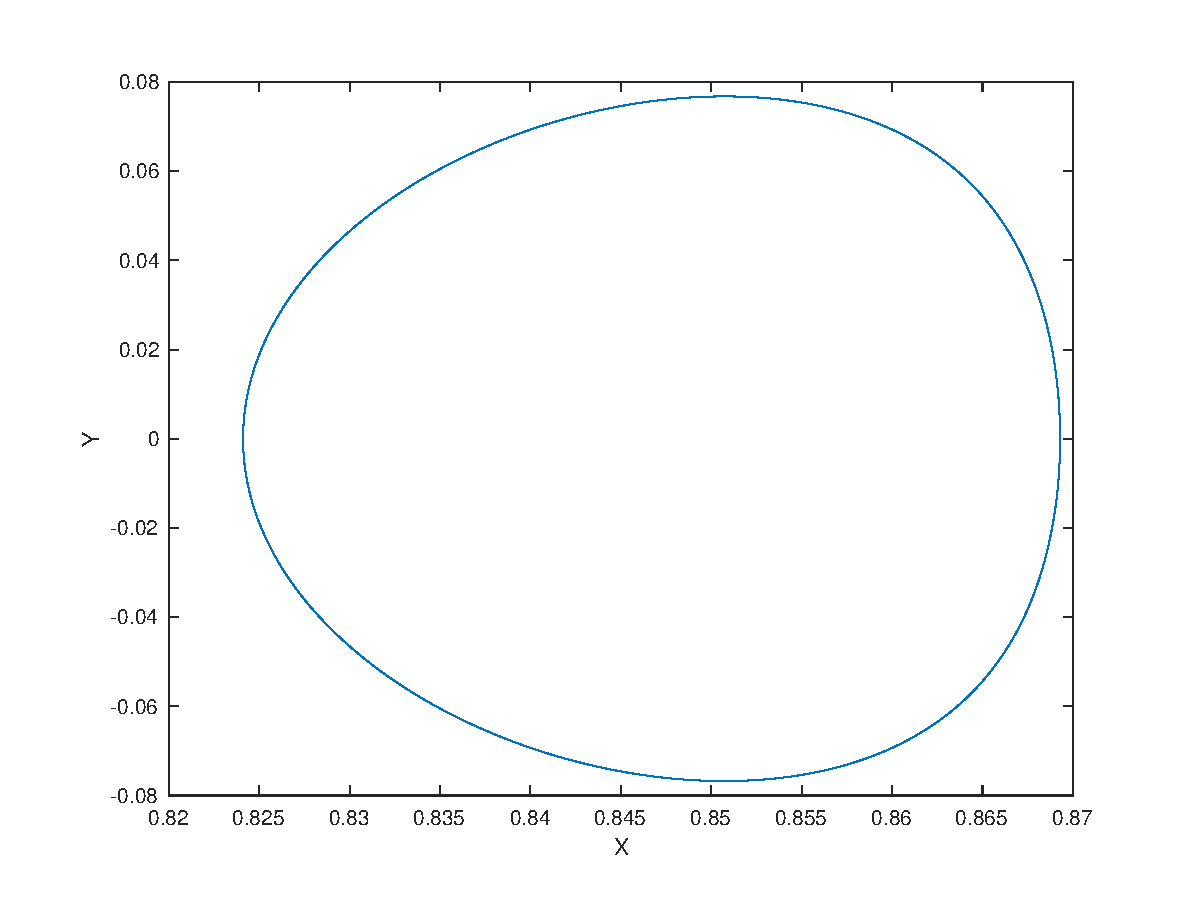
\includegraphics[width=\textwidth]{../Figure/Q2/fig4}
    \caption{Halo orbit in XY plane}
\end{figure}

\subsection{Part c}
In this section for adding perturbation we simulate halo orbit two times with about one percent of period time difference. Then two result are divided on we calculate the effect of perturbation on the orbit. The result is shown in the following figure:
\begin{figure}[H]
    \centering
    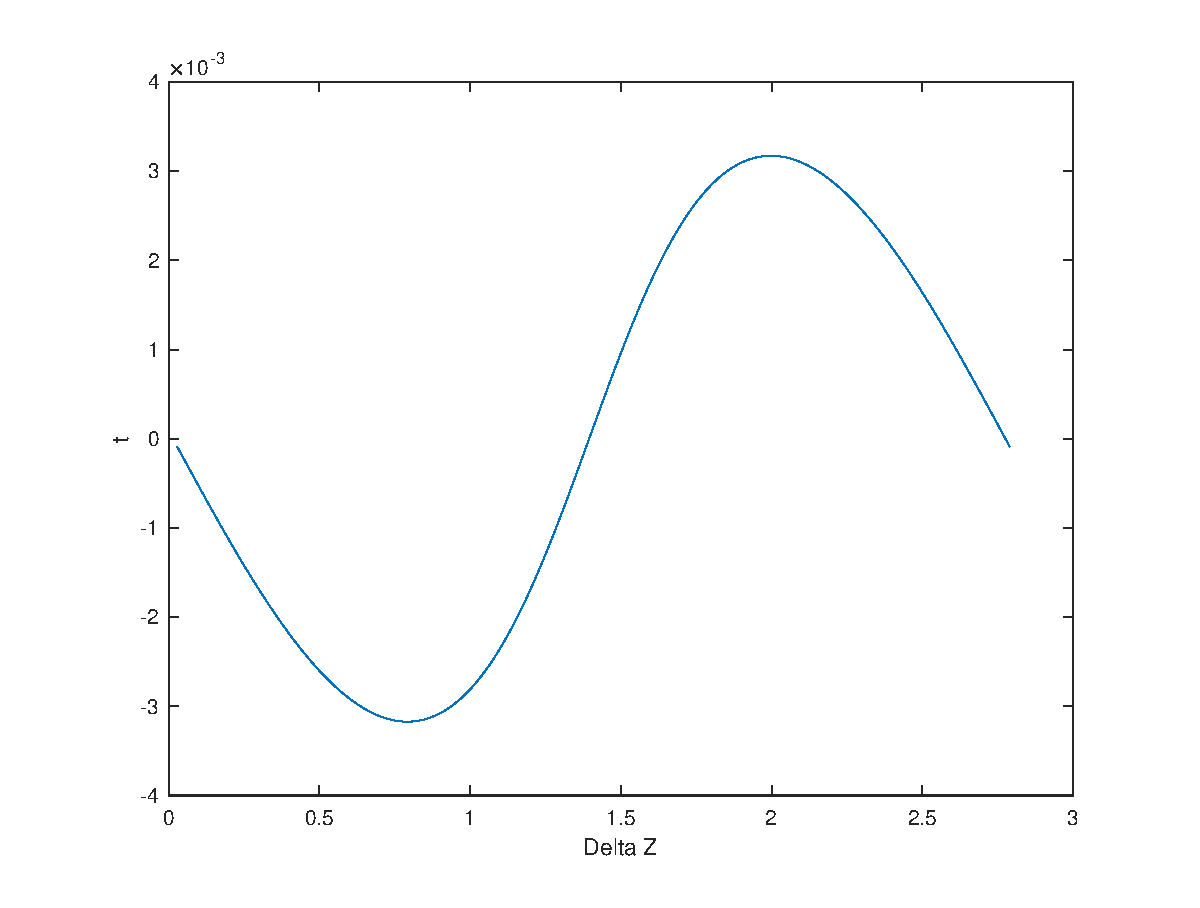
\includegraphics[width=\textwidth]{../Figure/Q2/Q2_1}
    \caption{Z difference over time}
\end{figure}

\begin{figure}[H]
    \centering
    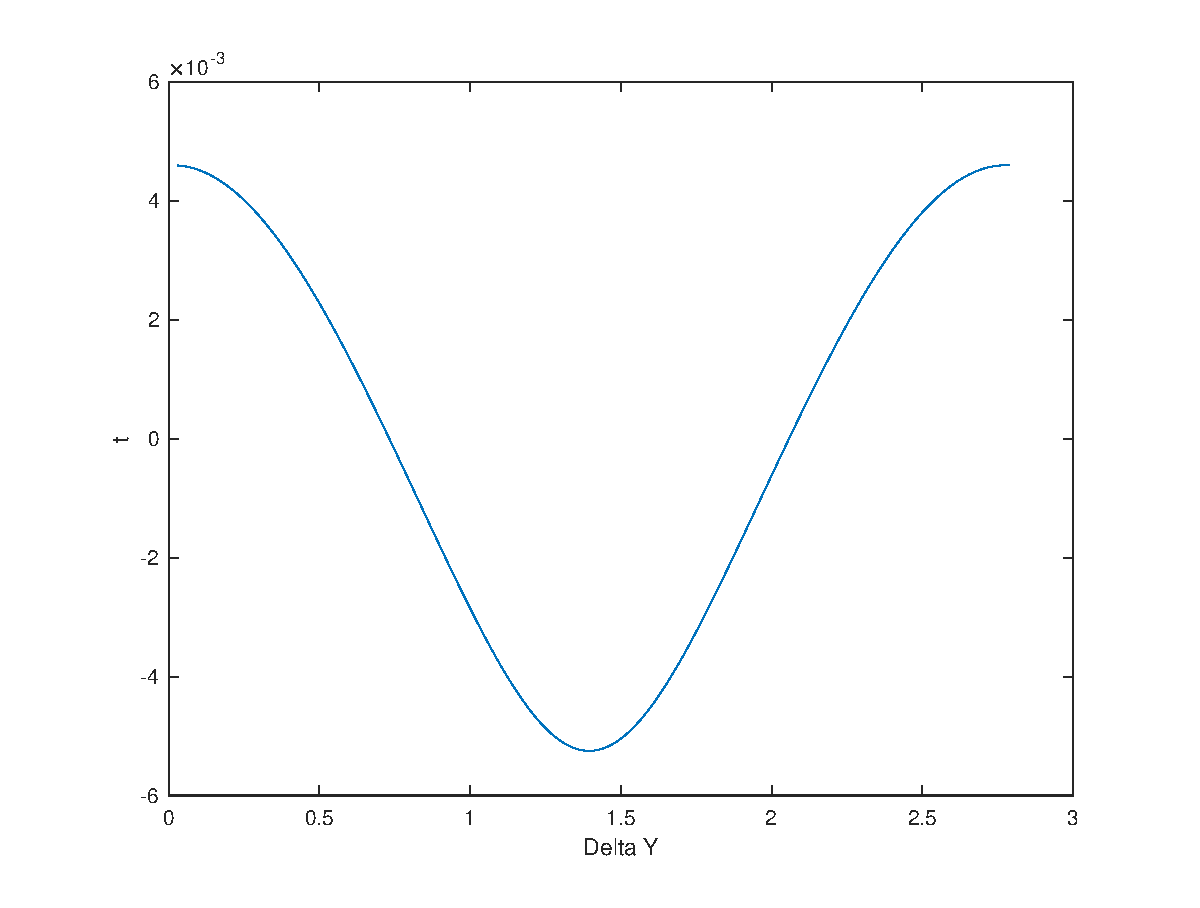
\includegraphics[width=\textwidth]{../Figure/Q2/Q2_2}
    \caption{Y difference over time}
\end{figure}

\begin{figure}[H]
    \centering
    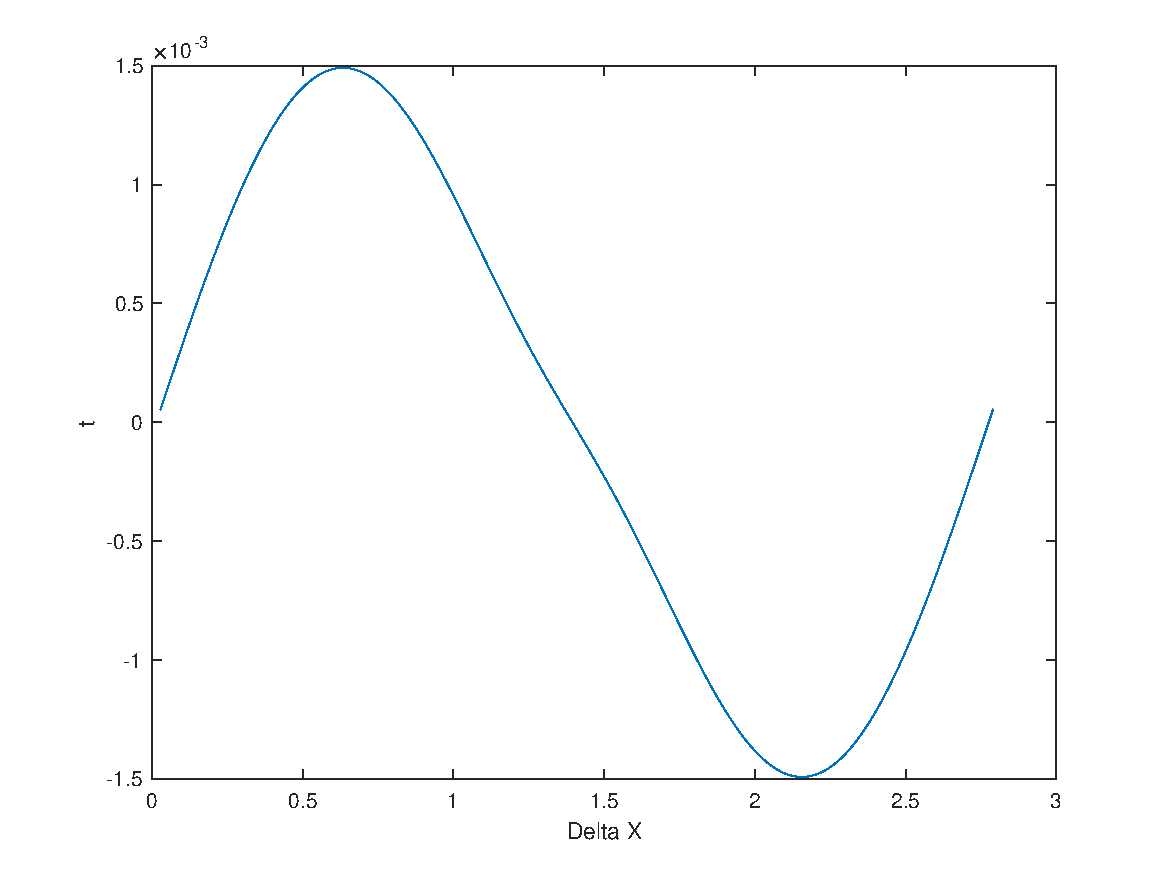
\includegraphics[width=\textwidth]{../Figure/Q2/Q2_3}
    \caption{X difference over time}
\end{figure}

From above result we can findout the orbit have marginal stability and have oscillating behavior. 